% ========================================
%	Header einbinden
% ========================================

\documentclass[bibtotoc,titlepage]{scrartcl}

% Deutsche Spracheinstellungen
\usepackage[ngerman,german]{babel, varioref}
\usepackage[T1]{fontenc}
\usepackage[utf8]{inputenc}

%\usepackage{marvosym}

\usepackage{amsfonts}
\usepackage{amssymb}
\usepackage{amsmath}
\usepackage{amscd}
\usepackage{amstext}

\usepackage{longtable}

%\usepackage{bibgerm}

\usepackage{footnpag}

\usepackage{ifthen}                 %%% package for conditionals in TeX
\usepackage[amssymb]{SIunits}
%Für textumflossene Bilder und Tablellen
%\usepackage{floatflt} - veraltet

%Für Testzwecke aktivieren, zeigt labels und refs im Text an.
%\usepackage{showkeys}

% Abstand zwischen zwei Absätzen nach DIN (1,5 Zeilen)
% \setlength{\parskip}{1.5ex plus0.5ex minus0.5ex}

% Einrückung am Anfang eines neuen Absatzes nach DIN (keine)
%\setlength{\parindent}{0pt}

% Ränder definieren
% \setlength{\oddsidemargin}{0.3cm}
% \setlength{\textwidth}{15.6cm}

% bessere Bildunterschriften
%\usepackage[center]{caption2}


% Problemlösungen beim Umgang mit Gleitumgebungen
\usepackage{float}

% Nummeriert bis zur Strukturstufe 3 (also <section>, <subsection> und <subsubsection>)
%\setcounter{secnumdepth}{3}

% Führt das Inhaltsverzeichnis bis zur Strukturstufe 3
%\setcounter{tocdepth}{3}
\usepackage[version=3]{mhchem}
	\mhchemoptions{minus-sidebearing-left=0.06em, minus-sidebearing-right=0.11em}
\usepackage{exscale}

\newenvironment{dsm} {\begin{displaymath}} {\end{displaymath}}
\newenvironment{vars} {\begin{center}\scriptsize} {\normalsize \end{center}}


\newcommand {\en} {\varepsilon_0}               % Epsilon-Null aus der Elektrodynamik
\newcommand {\lap} {\; \mathbf{\Delta}}         % Laplace-Operator
\newcommand {\R} { \mathbb{R} }                 % Menge der reellen Zahlen
\newcommand {\e} { \ \mathbf{e} }               % Eulersche Zahl
\renewcommand {\i} { \mathbf{i} }               % komplexe Zahl i
\newcommand {\N} { \mathbb{N} }                 % Menge der nat. Zahlen
\newcommand {\C} { \mathbb{C} }                 % Menge der kompl. Zahlen
\newcommand {\Z} { \mathbb{Z} }                 % Menge der kompl. Zahlen
\newcommand {\limi}[1]{\lim_{#1 \rightarrow \infty}} % Limes unendlich
\newcommand {\sumi}[1]{\sum_{#1=0}^\infty}
\newcommand {\rot} {\; \mathrm{rot} \,}         % Rotation
\newcommand {\grad} {\; \mathrm{grad} \,}       % Gradient
\newcommand {\dive} {\; \mathrm{div} \,}        % Divergenz
\newcommand {\dx} {\; \mathrm{d} }              % Differential d
\newcommand {\cotanh} {\; \mathrm{cotanh} \,}   %Cotangenshyperbolicus
\newcommand {\asinh} {\; \mathrm{areasinh} \,}  %Area-Sinus-Hyp.
\newcommand {\acosh} {\; \mathrm{areacosh} \,}  %Area-Cosinus-H.
\newcommand {\atanh} {\; \mathrm{areatanh} \,}  %Area Tangens-H.
\newcommand {\acoth} {\; \mathrm{areacoth} \,}  % Area-cotangens
\newcommand {\Sp} {\; \mathrm{Sp} \,}
\newcommand {\mbe} {\stackrel{\text{!}}{=}}     %Must Be Equal
\newcommand{\qed} { \hfill $\square$\\}
\renewcommand{\i} {\imath}
\def\captionsngerman{\def\figurename{\textbf{Abb.}}}

%%%%%%%%%%%%%%%%%%%%%%%%%%%%%%%%%%%%%%%%%%%%%%%%%%%%%%%%%%%%%%%%%%%%%%%%%%%%
% SWITCH FOR PDFLATEX or LATEX
%%%%%%%%%%%%%%%%%%%%%%%%%%%%%%%%%%%%%%%%%%%%%%%%%%%%%%%%%%%%%%%%%%%%%%%%%%%%
%%%
\ifx\pdfoutput\undefined %%%%%%%%%%%%%%%%%%%%%%%%%%%%%%%%%%%%%%%%% LATEX %%%
%%%
\usepackage[dvips]{graphicx}       %%% graphics for dvips
\DeclareGraphicsExtensions{.eps,.ps}   %%% standard extension for included graphics
\usepackage[ps2pdf]{thumbpdf}      %%% thumbnails for ps2pdf
\usepackage[ps2pdf,                %%% hyper-references for ps2pdf
bookmarks=true,%                   %%% generate bookmarks ...
bookmarksnumbered=true,%           %%% ... with numbers
hypertexnames=false,%              %%% needed for correct links to figures !!!
breaklinks=true,%                  %%% breaks lines, but links are very small
linkbordercolor={0 0 1},%          %%% blue frames around links
pdfborder={0 0 112.0}]{hyperref}%  %%% border-width of frames
%                                      will be multiplied with 0.009 by ps2pdf
%
\hypersetup{ pdfauthor   = {Hannes Franke; Julius Tilly},
pdftitle    = {V301 Innenwiderstand und Leistungsanpassung}, pdfsubject  = {Protokoll FP}, pdfkeywords = {V301, Innenwiderstand, Leistungsanpassung},
pdfcreator  = {LaTeX with hyperref package}, pdfproducer = {dvips
+ ps2pdf} }
%%%
\else %%%%%%%%%%%%%%%%%%%%%%%%%%%%%%%%%%%%%%%%%%%%%%%%%%%%%%%%%% PDFLATEX %%%
%%%
\usepackage[pdftex]{graphicx}      %%% graphics for pdfLaTeX
\DeclareGraphicsExtensions{.pdf}   %%% standard extension for included graphics
\usepackage[pdftex]{thumbpdf}      %%% thumbnails for pdflatex
\usepackage[pdftex,                %%% hyper-references for pdflatex
bookmarks=true,%                   %%% generate bookmarks ...
bookmarksnumbered=true,%           %%% ... with numbers
hypertexnames=false,%              %%% needed for correct links to figures !!!
breaklinks=true,%                  %%% break links if exceeding a single line
linkbordercolor={0 0 1},
linktocpage]{hyperref} %%% blue frames around links
%                                  %%% pdfborder={0 0 1} is the default
\hypersetup{
pdftitle    = {V301 Innenwiderstand und Leistungsanpassung}, 
pdfsubject  = {Protokoll AP}, 
pdfkeywords = {V301, Innenwiderstand, Leistungsanpassung},
pdfsubject  = {Protokoll AP},
pdfkeywords = {V301, Innenwiderstand, Leistungsanpassung}}
%                                  %%% pdfcreator, pdfproducer,
%                                      and CreationDate are automatically set
%                                      by pdflatex !!!
\pdfadjustspacing=1                %%% force LaTeX-like character spacing
\usepackage{epstopdf}
%
\fi %%%%%%%%%%%%%%%%%%%%%%%%%%%%%%%%%%%%%%%%%%%%%%%%%%% END OF CONDITION %%%
%%%%%%%%%%%%%%%%%%%%%%%%%%%%%%%%%%%%%%%%%%%%%%%%%%%%%%%%%%%%%%%%%%%%%%%%%%%%
% seitliche Tabellen und Abbildungen
%\usepackage{rotating}
\usepackage{ae}
\usepackage{
  array,
  booktabs,
  dcolumn
}
\makeatletter 
  \renewenvironment{figure}[1][] {% 
    \ifthenelse{\equal{#1}{}}{% 
      \@float{figure} 
    }{% 
      \@float{figure}[#1]% 
    }% 
    \centering 
  }{% 
    \end@float 
  } 
  \makeatother 


  \makeatletter 
  \renewenvironment{table}[1][] {% 
    \ifthenelse{\equal{#1}{}}{% 
      \@float{table} 
    }{% 
      \@float{table}[#1]% 
    }% 
    \centering 
  }{% 
    \end@float 
  } 
  \makeatother 
%\usepackage{listings}
%\lstloadlanguages{[Visual]Basic}
%\allowdisplaybreaks[1]
%\usepackage{hycap}
%\usepackage{fancyunits}


% ========================================
%	Angaben für das Titelblatt
% ========================================

\title{Versuch 406 - Beugung am Spalt\\				% Titel des Versuchs 
\large TU Dortmund, Fakultät Physik\\ 
\normalsize Anfänger-Praktikum}

\author{Jan Adam\\			% Name Praktikumspartner A
{\small \href{jan.adam@tu-dortmund.de}{jan.adam@tu-dortmund.de}}	% Erzeugt interaktiven einen Link
\and						% um einen weiteren Author hinzuzfügen
Dimitrios Skodras\\					% Name Praktikumspartner B
{\small \href{dimitrios.skodras@tu-dortmund.de}{dimitrios.skodras@tu-dortmund.de}}		% Erzeugt interaktiven einen Link
}
\date{30.Oktober 2012}				% Das Datum der Versuchsdurchführung

% ========================================
%	Das Dokument beginnt
% ========================================

\begin{document}

% ========================================
%	Titelblatt erzeugen
% ========================================

\maketitle					% Jetzt wird die Titelseite erzeugt
\thispagestyle{empty} 				% Weder Kopfzeile noch Fußzeile

% ========================================
%	Der Vorspann
% ========================================

%\newpage					% Wenn Verzeichnisse auf einer neuen Seite beginnen sollen
%\pagestyle{empty}				% Weder Kopf- noch Fußzeile für Verzeichnisse

\tableofcontents

%\newpage					% eine neue Seite
%\thispagestyle{empty}				% Weder Kopf- noch Fußzeile für Verzeichnisse
%\listoffigures					% Abbildungsverzeichnis

%\newpage					% eine neue Seite
%\thispagestyle{empty}				% Weder Kopf- noch Fußzeile für Verzeichnisse
%\listoftables					% Tabellenverzeichnis
\newpage					% eine neue Seite


% ========================================
%	Kapitel
% ========================================

\section{Einleitung}				% Bei Bedarf
Wenn physikalische Wellen, wie Wasserwellen, Schall oder Licht auf ein Hindernis mit einem Spalt treffen, dessen Durchmesser 
klein gegen die Wellenlänge ist, tritt das Phänomen der Beugung auf (auch Diffraktion genannt). Man wird dabei zwar dem
tatsächlichen Charakter elektromagnetischer Wellen nicht gerecht, doch durch Mittelung über eine Großzahl von Photonen, ist
das klassische Wellenmodell geeignet. Die Beugung von Licht wird im Zuge des Experiments an einem Einfachspalt fester Breite, einem Einfachspalt variabler Breite, sowie an einem Doppelspalt
betrachtet.

\section{Theorie}
Die Fresnelsche Beugung beschreibt den Fall, bei dem sowohl Lichtquelle als auch Abbildungsschirm im Endlichen liegen und daher die Wellen,
die in P interferieren, mit unterschiedlichen Winkeln $\phi_1$ und $\phi_2$ gebeugt werden. Da das mathematisch komplexere
Beschreibungen erfordert, ist die Fraunhofersche Betrachtung leichter in der Handhabung. Hier wird sowohl das ein- als auch das ausfallende Licht als parallel angesehen und die Überlagerung durch eine hypothetische Sammellinse ermöglicht. Das parallele Lichtbündel wird
hierbei durch die Verwendung eines Lasers ermöglicht. Zur Verhinderung von Kugelwellen und damit zur Beschränkung der
Dimension, ist es notwendig, dass die Spaltbreite $b$ klein gegen seine Länge ist.


\begin{figure}[htbp]
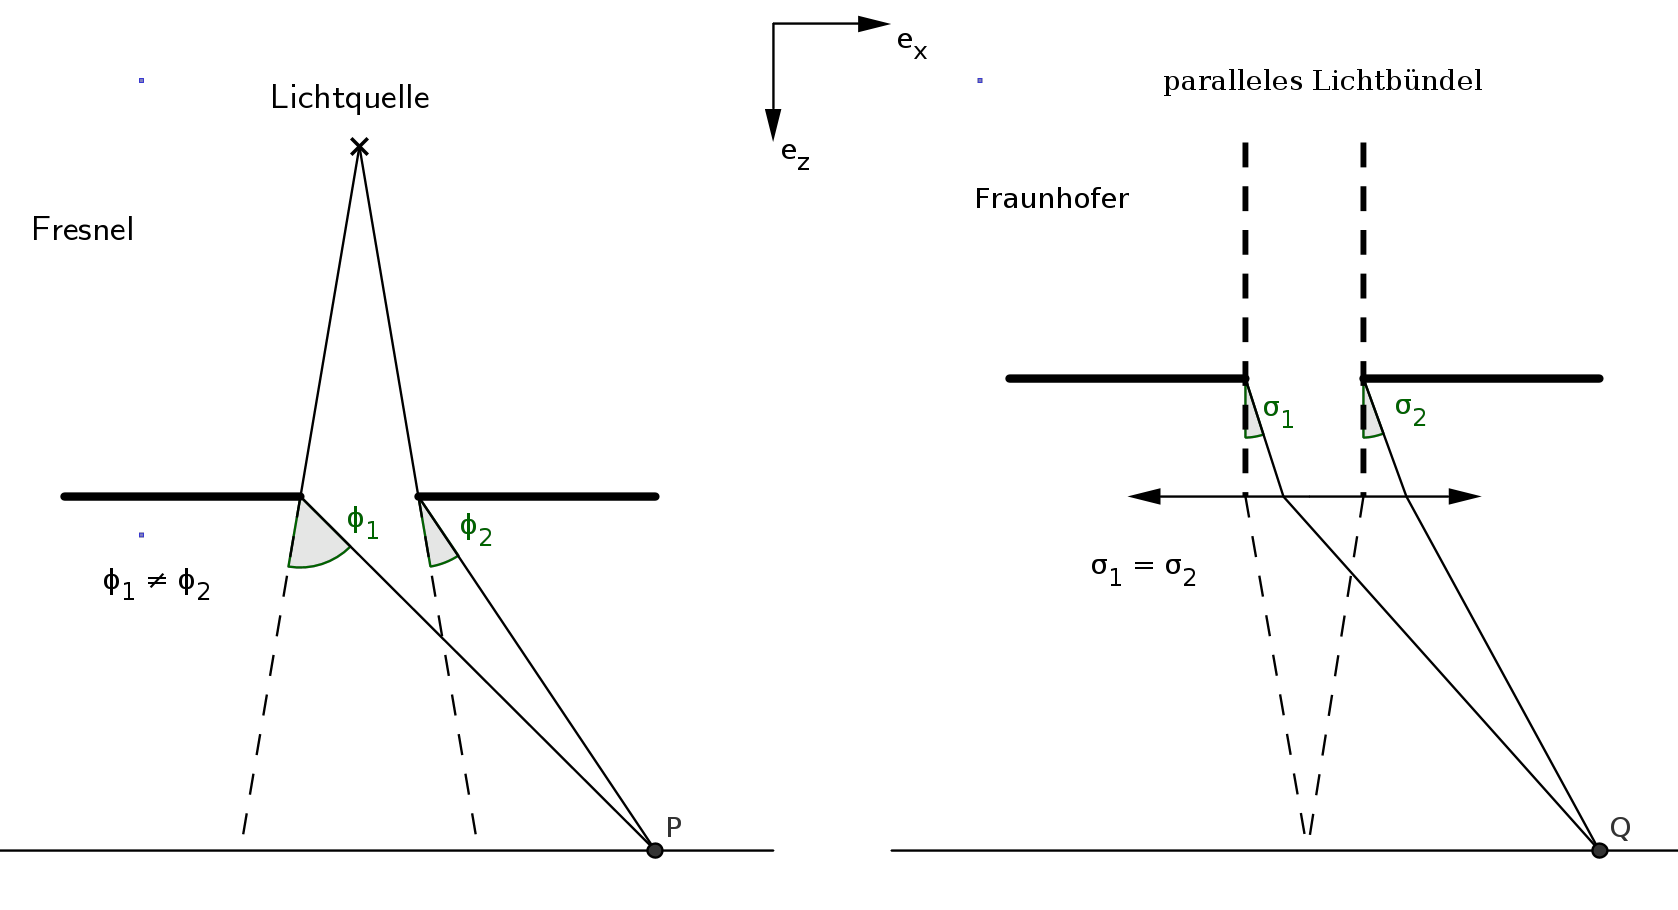
\includegraphics[width=1\textwidth]{pics/406_1.png}
\centering
\caption {Fresnelsche und Fraunhofersche Beugung}
\end{figure}


Voraussetzung zur Erklärung der Intereferenzmuster ist das huygens-fresnelsche Prinzip. Es besagt, dass jeder Punkt einer
Wellenfront Ausgangspunkt einer neuen Welle ist. Durch Superposition, oder eben Interferenz, der Elementarwellen entsteht
die neue Wellenfront.

\subsection{Mathematische Beziehungen - Einfachspalt}
Eine ebene Welle falle in parallel zu $\vec{e}_z$ auf den Spalt ein. Pro Längeneinheit der Wellenfront habe sie eine Feldstärke,
ausgedrückt durch

\begin{align}
 A(z,t) = A_0 \exp[i(\omega t - kz)], \quad \text{mit} \quad  k =  \frac{2\pi}{\lambda}.
\label{Wellenfront} 
\end{align}

Da die am Spalt entstehenden Wellen, die in Punkt Q miteinander interferieren, nicht alle denselben Gangunterschied $\Delta s$ haben, 
sind die Winkel, unter denen sie dort auftreffen, ebenfalls unterschiedlich. 


\begin{align}
 \delta = \frac{2\pi \Delta s}{\lambda} = \frac{2\pi x \sin(\phi)}{\lambda}.
\label{delta} 
\end{align}

Da die Feldstärke $B(z,t,\phi)$ aus der Integration über sämtliche Feldstärken $A(z,t,\delta)$ \eqref{Wellenfront} mit genannten Phasendifferenzen \eqref{delta}
entlang der Spaltenbreite von 0 bis $b$ hervorgeht, ergibt sich unter noch hinzugezogener Eulerschen Formel folgender Ausdruck:

\begin{align*}
 B(z,t,\phi) & = A_0 \int\limits_0^b exp[i(\omega t - kx + \delta) \\
 & = A_0 exp \left[ i \left( \omega t - \frac{2\pi z}{\lambda} + \eta \right) \right] \cdot \frac{\lambda \sin(\eta)}{\pi \sin(\phi)}, \quad \text{mit} \quad \eta = \frac{\pi b \sin(\phi)}{\lambda}.
\notag
\end{align*}


Das löst zwar das Problem, aber für die experimentelle Überprüfung genügen die letzten beiden Anteile, sodass sich verkürzt ergibt


\begin{align}
 B(\phi) = A_0 b \frac{sin(\eta)}{\eta}.
\label{B}
\end{align}

Diese Funktion ist achsensymmetrisch an der y-Achse und hat Nulldurchgänge bei $\sin(\phi_n) = \pm  \frac{\lambda}{b}$ \quad \text{mit} \quad $n \in \mathbb {N}$.
Aufgrund der hohen Frequenz von Licht mit einer Größenordnung von $10^{14}$ Hz, ist eine direkte Messung nicht möglich und
daher weicht man auf die zeitlich gemittelte Intensität $I(\phi)$ aus

\begin{align*}
 I(\phi) \propto B(\phi)^2 = A_0^2 b^2 \left( \frac{\lambda \sin(\eta)}{\pi b \sin(\phi)} \right)^2.
\notag
\end{align*}


$I$ hat nun dort Minima, wo $B$ Nulldurchgänge hat. Die Werte der Maxima nehmen in etwa quadratisch mit dem Beugungswinkel ab.

\subsection{Mathematische Beziehungen - Doppelspalt}
Das Beugungsverhalten am Doppelspalt gestaltet sich wie die Überlagerung zweier Einfachspalte der Spaltenbreite $b$ und einem Abstand $s$ zueinander.


\begin{figure}[htbp]
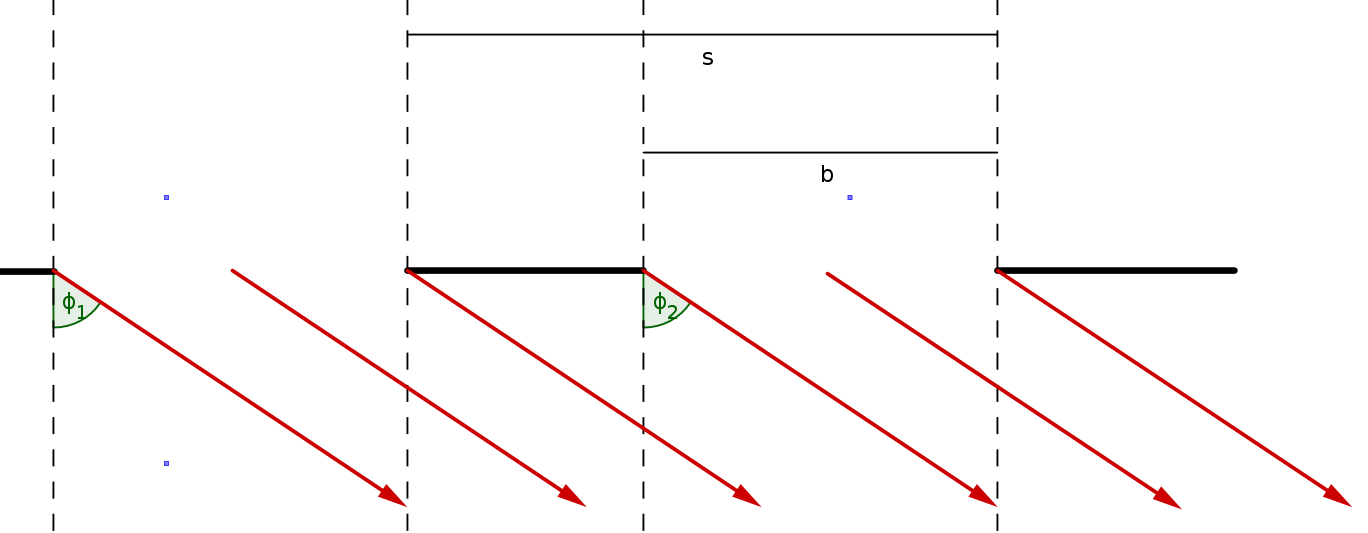
\includegraphics[width=1\textwidth]{pics/406_2.png}
\centering
\caption {Beugung am Doppelspalt}
\end{figure}


Die Intesitätsverteilung am Doppelspalt ergibt sich aus der Intensitätsverteilung des Einzelspaltes und einer $\cos^2$-Verteilung zu

\begin{align*}
 I(\phi) \propto B(\phi)^2 = 4 \cos^2 \left( \frac{\pi s \sin(\eta)}{\lambda} \right) \cdot \left(\frac{\sin(\eta)}{\eta} \right)^2.
\notag
\end{align*}

Zusätzliche Minima aus der $\cos^2$-Verteilung entstehen an den Stellen $\phi(n)= \lambda \arcsin(\frac{2n+1}{2s})$ mit $n \in \mathbb{N}_0$

\subsection{Fraunhofersche Beugung und Fourier-Transformation}
Durch eine Fouriertransformation der Funktion aus \eqref{Wellenfront} kann man als $B(\phi)$ ansehen. Allgemein hat eine fouriertransformierte
Funktion $f(x)$ folgendes Aussehen:

\begin{align}
 g(\xi) := \int\limits_{-\infty}^{+\infty} f(x) \mathrm{e}^{ix\xi}dx, \intertext{mit} 
  \label{fourier}
  f(x) =\begin{cases}
        A_0, & 0 \leq x \leq b\\
        0, & \text{sonst} \qquad .
        \nonumber
       \end{cases}
\end{align}

Nach wiederholter Anwendung der Eulerschen Formel, sowie der Definition von \\ $\xi = \frac{2\pi \sin(\phi)}{\lambda} = \frac{2 \eta}{b}$
finden wir die Übereinstimmung zwischen \eqref{B} und (4). Damit ist gezeigt, dass das huygenssche-fresnelsche Prinzip durch
die Fouriertransformation mathematisch beschrieben wird. Der Phasenfaktor $\mathrm{e}^{ix\xi}$ beschreibt gerade die Phasendifferenz,
einer Welle, die von $x$ ausgeht bezüglich der in $x=0$ emitierten Welle.

\section{Durchführung}
Mit einem Helium-Neon-Laser mit einer Wellenlänge von $\lambda = 633$ nm werden verschiedene Spaltbilder bestrahlt.
Auf der Abbildung rechts vom Spalt ist in einer Entfernung von $L\approx 100$ cm ein zur optischen Achse senkrecht 
verschiebbarer Detektor aufgebaut. Mit der Photodiode darin lässt sich das Beugungsbild aufnehmen.

\begin{figure}[htbp]
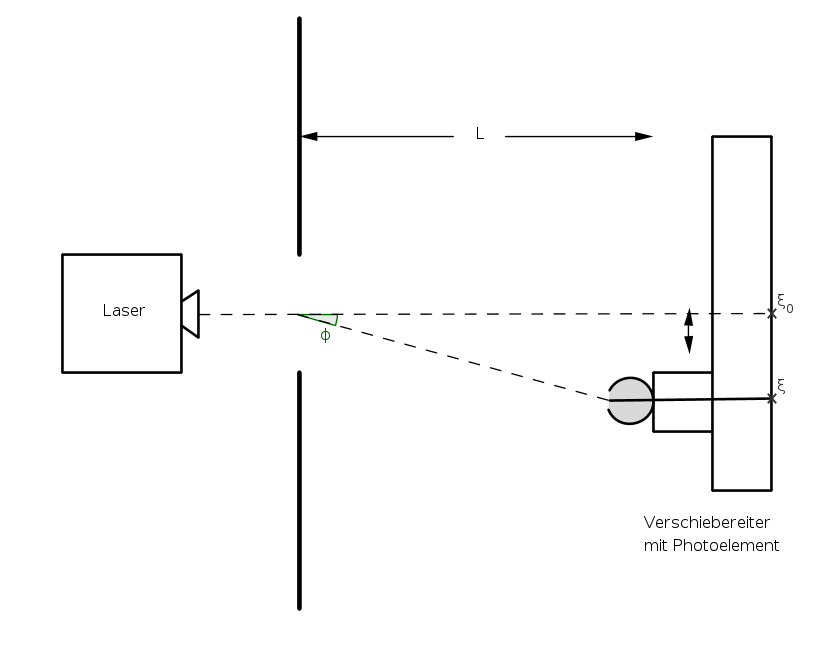
\includegraphics[height=8.5cm]{pics/406_3.png}
\centering
\caption{Versuchsaufbau}
\end{figure}

\section{Auswertung}
Die Messdaten werden in einer Tabelle aufgetragen und mit dem Grafikprogramm gnuplot ausgewertet. In den folgenden Grafiken finden sich alle Messpunkte und eine, an die Spaltparameter angepasste, Kurve, die den theoretischen Verlauf der Messwerte darstellen soll. Die Spaltparameter wurden aus den Messwerten errechnet, indem die Kurve so angepasst wurde, dass sie die kleinstmögliche Abweichung zu den Messwerten hat.\\
Gemessen wurde die Beugungsfigur an insgesamt 50 Messpunkten im Abstand von 0,5 mm ausgehend vom Nullpunkt entlang der positiven x-Achse. Die Punkte auf der linken Seite sind die an der y-Achse gespiegelten Messwerte, die dazu dienen, dass man die Beugungsfiguren besser erkennen kann.

\begin{figure}[htbp]
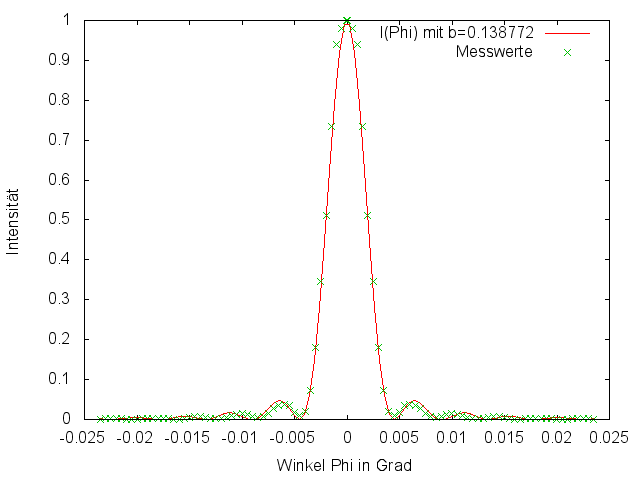
\includegraphics[width=12cm]{pics/1.png}
\centering
\label{a1}
\caption{Einfachspalt gefittet}
\end{figure}

\begin{figure}[htbp]
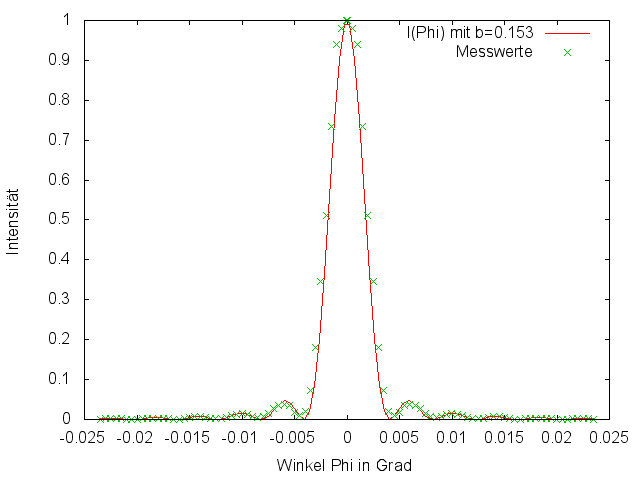
\includegraphics[width=12cm]{pics/3.png}
\centering
\label{a2}
\caption{Einfachspalt eigene Parameter}
\end{figure}


\begin{figure}[htbp]
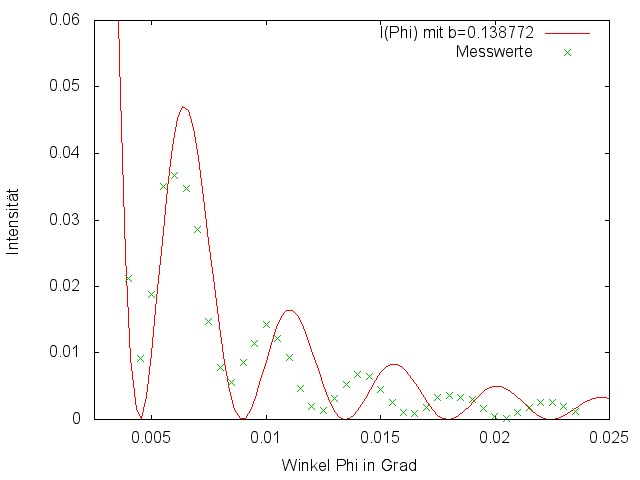
\includegraphics[width=12cm]{pics/2.png}
\centering
\label{a3}
\caption{Einfachspalt gefittet kleinerer Ausschnitt}
\end{figure}

\begin{figure}[htbp]
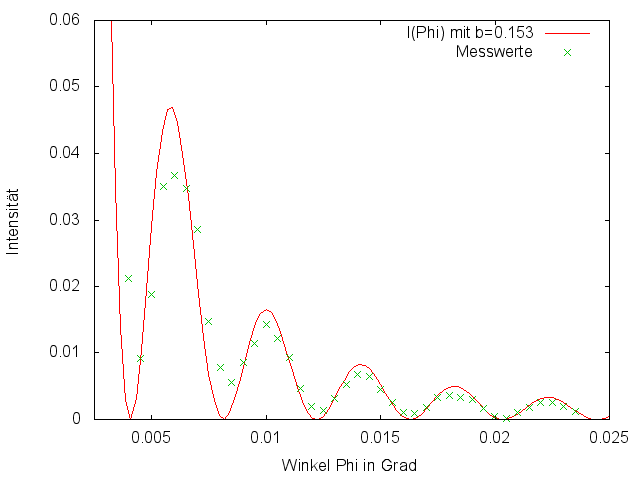
\includegraphics[width=12cm]{pics/4.png}
\centering
\label{a4}
\caption{Einfachspalt eigene Parameter kleinerer Ausschnitt}
\end{figure}


\begin{figure}[htbp]
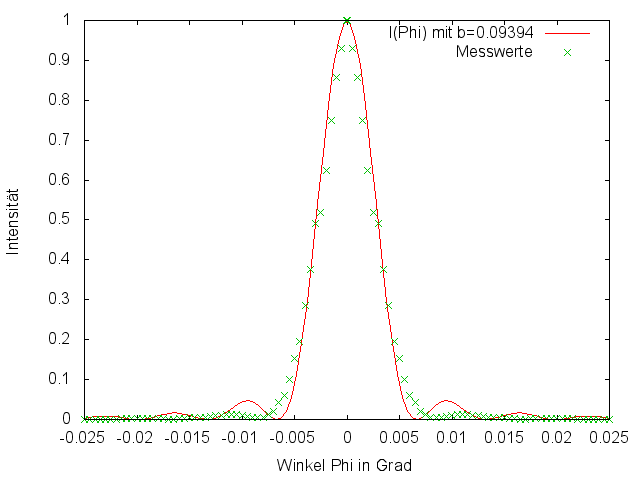
\includegraphics[width=12cm]{pics/5.png}
\centering
\label{a5}
\caption{Variabler Einfachspalt gefittet}
\end{figure}

\begin{figure}[htbp]
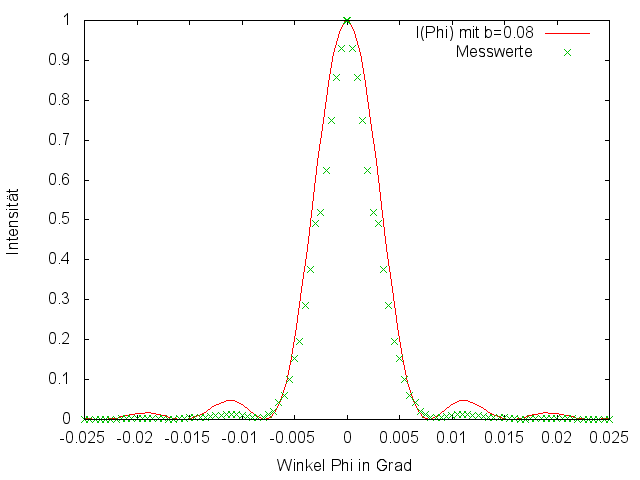
\includegraphics[width=12cm]{pics/7.png}
\centering
\label{a6}
\caption{Variabler Einfachspalt eigene Parameter}
\end{figure}


\begin{figure}[htbp]
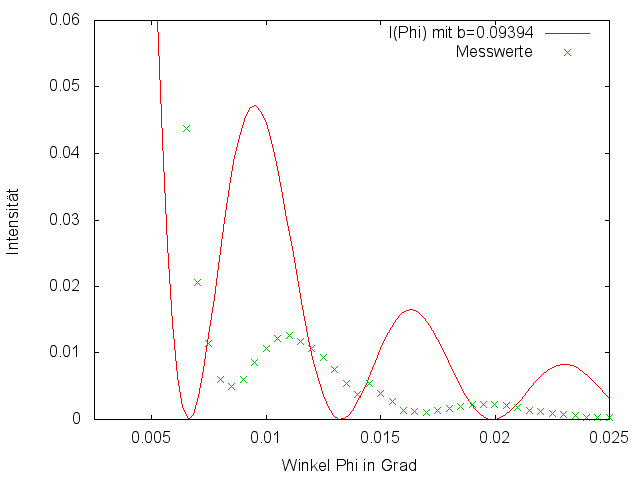
\includegraphics[width=12cm]{pics/6.png}
\centering
\label{a7}
\caption{Variabler Einfachspalt gefittet kleinerer Ausschnitt}
\end{figure}

\begin{figure}[htbp]
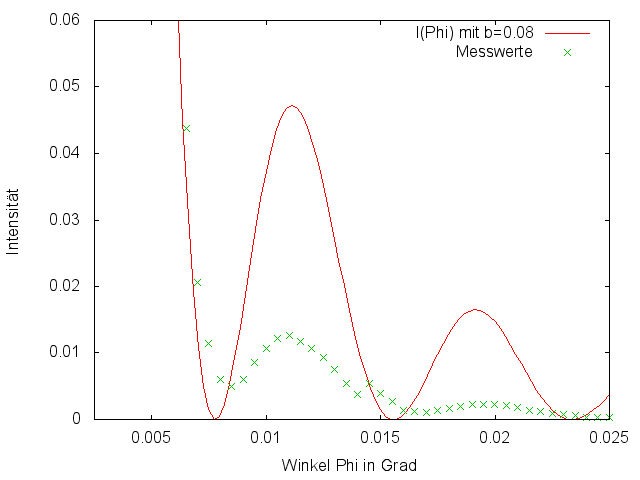
\includegraphics[width=12cm]{pics/8.png}
\centering
\label{a8}
\caption{Variabler Einfachspalt eigene Parameter kleinerer Ausschnitt}
\end{figure}


\begin{figure}[htbp]
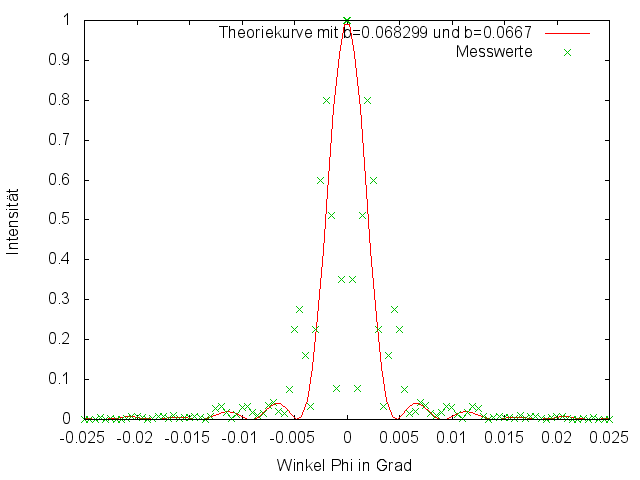
\includegraphics[width=12cm]{pics/9.png}
\centering
\label{a9}
\caption{Doppelspalt gefittet}
\end{figure}

\begin{figure}[htbp]
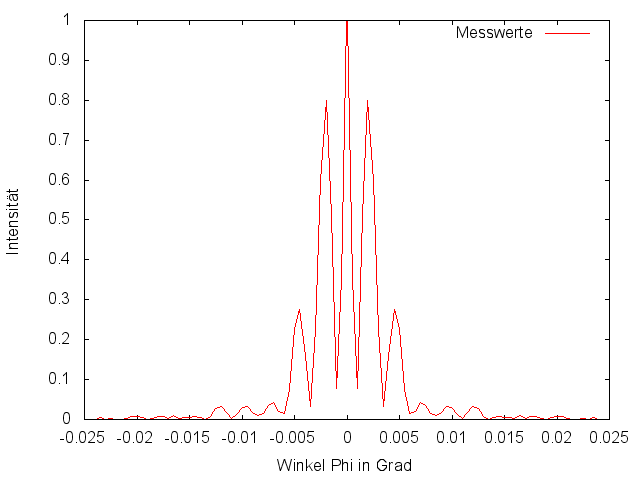
\includegraphics[width=12cm]{pics/10.png}
\centering
\label{a10}
\caption{Doppelspalt Messwerte mit Linien}
\end{figure}


\begin{figure}[htbp]
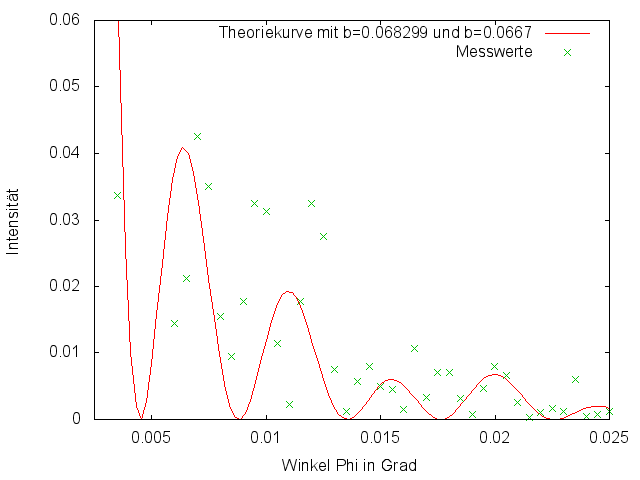
\includegraphics[width=12cm]{pics/11.png}
\centering
\label{a11}
\caption{Doppelspalt gefittet kleinerer Ausschnitt}
\end{figure}

\subsection{Einfachspalt feste Breite}
Beim Einfachspalt mit fester Breite ergab die Auswertung einen idealen Wert von 0,138772 mm für die Spaltbreite b. Abbildung 4 und Abbildung 6 zeigen die Messwerte und die entsprechend geplotteten Funktionen. Abbildung 6 zeigt dabei einen kleineren Ausschnitt, der die Extrema höherer Ordnung besser auflöst.\\
Bei der Wahl von 0,15 mm für b ergab sich eine Kurve wie in Abbildung 5 und Abbildung 7 dargestellt.\\

\subsection{Einfachspalt variable Breite}
Beim Einfachspalt mit variabler Spaltbreite errechnete das Programm einen Wert von 0,09394 mm für die Spaltbreite b. Abbildung 8 und Abbildung 10 zeigen die Messwerte und die entsprechend geplotteten Funktionen. Abbildung 10 zeigt dabei wieder eine Vergrößerung der Extrema höherer Ordnung.\\
Bei der Wahl von 0,08 mm für b ergab sich eine Kurve wie in Abbildung 9 und Abbildung 11 dargestellt.\\

\subsection{Doppelspalt}
Abbildung 12 bis 14 zeigt die Beugungsfigur des Doppelspaltes bei einer Spaltbreite von , wobei in Abbildung 13 nur die Messwerte durch linien verbunden aufgetragen sind und die anderen beiden Abbildungen wieder eine Gesamtaufnahme und eine Vergrößerung der Daten mit Theoriekurve beinhalten.

\subsection{Verwendung des Mikroskops}
Um das Mikroskop zur Ausmessung der Spaltbreite verwenden zu können, muss dieses zuvor geeicht werden. Im Okular ist ein Raster eingelassen, wodurch Objektgrößen in Rastereinheiten vermessen werden können. Da die Rastereinheiten jedoch je nach Vergrößerung anderen Abständen auf dem Präparat entsprechen, wird mit einer kleinen Millimeterskala die Größe der Einheiten in der aktuellen Zoomstufe bestimmt.\\
Als Eichwert ergab sich, dass eine Länge von 10 Längeneinheiten [LE] eine Länge von 3,52 mm entspricht.\\
Bei einer Spaltbreite von $0,46\pm 0,1$ LE ergibt dies durch Verwendung des Dreisatzes eine Spaltbreite von $0,16192\pm 0.0352 $ mm\\
Die gemessene Spaltbreite passt sehr gut zu der vom Hersteller angegebenen Breite von 0,16 mm. 

\section{Diskussion}
Wie zu erkennen ist, weichen die Theoriekurven teils signifikant von den Messwerten ab. Dies ist in erster Linie auf Messungenauigkeiten zurückzuführen. Da der Raum nicht vollständig verdunkelt war, beinhalten alle Messwerte einen Dunkelstrom in der Größenordnung von 0,01 nA. Dieser ist zwar verschwindend gering, aber zusätzlich haben externe Lichtquellen die Messungen unregelmäßig beeinflusst, so dass die Theoriekurve nicht vollständig an die Messwerte anliegen kann.
Die Abweichungen sind jedoch erst im Bereich der Extrema höherer Ordnung entsprechend groß, so dass davon ausgegangen werden kann, dass die Photodiode auf so kleinen Skalen nicht mehr genau genug arbeitet.

Zusätzlich darf davon ausgegangen werden, dass gnuplot zwar die geringste Abweichung in y-Richtung bestimmt, diese jedoch aufgrund der doch relativ wenigen Messpunkte nicht unbedingt die Ergebnisse widerspiegelt. Insbesondere bei den Maxima höherer Ordnung weichen die gefitteten Kurven sehr stark von den Messwerten ab, was daran liegt, dass gnuplot offenbar mit absoluten Abweichungen rechnet und diese sind bei den Maxima höherer Ordnung natürlich deutlich geringer. Daher wird die Funktion eher am ersten Hauptmaximum angelegt, von dem aber nur relativ wenige Messpunkte vorliegen. Wenn man die starke Steigung der Kurve am ersten Maximum betrachtet, wäre es günstiger gewesen, dort Messwerte mit einer größeren Dichte aufzunehmen.\\

Betrachtet man die Extrema höherer Ordnung und variiert den Wert von b so, dass die Extrema nun übereinander liegen, so ergeben sich für den festen und den variablen Einzelspalt neue Spaltbreiten von 0,153 mm bzw. 0,08 mm, wodurch die Kurven zwar etwas stärker vom ersten Maximum abweichen, aber qualitativ deutlich besser zum Beugungsbild passen.
Da die Intensitätsmessung relativ ungenau ausgefallen ist, erscheint es sinnvoller, sich eher an dem Winkel der Maxima zu orientieren, als am Fehler deren Intensität. Denn die Position kann auch bei ungenauerer Amplitude immer noch sehr genau gemessen werden. Deshalb sind die selbstgewählten Werte die repräsentativen.\\

Im Falle des festen Spaltes passen diese auch viel besser zum tatsächlichen Wert von 0,16 mm.
Der selbstgewählte Wert weicht hier um 4,375\% vom tatsächlichen ab, während der gefittete Wert eine Abweichung von 13,2675\% aufweist.\\

Die Kurve des Doppelspalts zeigen eine starke Abweichung von den Messwerten. Während die Messwerte wieder ein zentrales Maximum und danach weiter stark ausgeprägte Maxima anzeigt, sieht die Fitfunktion wie beim Einzelspalt aus. Auch bei den Maxima höherer Ordnung gibt es starke Abweichungen, die nur darauf zurückführbar sein können, dass im Bereich um das erste Maximum zu wenig Messwerte aufgenommen wurden. Selbst mit bloßem Auge ist kein Muster im Verlauf der Messwerte erkennbar, erst wenn alle Punkte durch Linien miteinander verbunden werden, kann man sich davon überzeugen, dass das charakteristische Doppelspaltbild vermessen wurde.

Zusammenfassend kann man sagen, dass die Messung mit dem Mikroskop deutlich einfacher und auch aussagekräftiger ist, als die Methode der Beugungsbildanalyse, da die Theoriekurve der errechneten Werte doch sehr stark von den Messpunkten abweicht. Da die selbstgewählten Werte keine Sicherheit durch irgendwelche Auswertungen haben, sind auch diese nicht ausreichend gesichert. Würde die Fitfunktion mit einer relativen Abweichung arbeiten, wären die gefitteten Werte jedoch  möglicherweise brauchbarer.\\

Vorausgesetzt, dass dann in etwa die selben Werte herauskommen würden, wie die selbst nach Augenmaß bestimmten, würden beide Methoden in etwa gleich gute Ergebnisse erzielen.\\
Beide Methoden sind jedoch deutlich Fehlerbehaftet, da die Messung derart schwacher Lichtsignale schwierig ist, und das Raster im Mikroskop viel zu grob ist, um genaue Werte zu erhalten.


\tt{blabla}
% ========================================
%	Literaturverzeichnis
% ========================================

%\bibliographystyle{plainnat}			% Bibliographie-Style auswählen
%\bibliography{BIBDATEI}			% Literaturverzeichnis

% ========================================
%	Das Dokument endent
% ========================================

\end{document}
